%!TEX TS-program = xelatex
\documentclass{friggeri-cv}
\usepackage{afterpage}
\usepackage{hyperref}
\usepackage{color}
% \usepackage[style=apa]{biblatex}
\usepackage{xcolor}
\hypersetup{
    pdftitle={},
    pdfauthor={},
    pdfsubject={},
    pdfkeywords={},
    colorlinks=false,       % no lik border color
   allbordercolors=white    % white border color for all
}
\usepackage{longtable}
\usepackage{tabularx}
\addbibresource{talks.bib}
\addbibresource{articles.bib}
\addbibresource{code.bib}
\addbibresource{posters.bib}
\RequirePackage{xcolor}
\definecolor{pblue}{HTML}{505050}
\usepackage{emptypage}
\newlength\tdima
\newcommand\tabfill[1]{%
      \setlength\tdima{\linewidth}%
      \addtolength\tdima{\@}%
      \addtolength\tdima{-\dimen\@}%
      \parbox[t]{\tdima}{#1\ifhmode\strut\fi}}
\hypersetup{pdfborder = 0 0 0}
\newcommand\mytabs{\hspace*{1cm}\=\hspace{1cm}\=\hspace{2cm}}
\newenvironment{mysec}[1][\mytabs]
  {\begin{tabbing}#1\kill\ignorespaces}
  {\end{tabbing}}
\begin{document}
\header{\hspace{5mm}\Huge{Thomas J.}}{ \Huge{Maullin-Sapey}}
      {\hspace{5cm} Researcher in Neuroimaging Statistics}
      
% Fake text to add separator      
\fcolorbox{white}{gray}{\parbox{\dimexpr\textwidth-2\fboxsep-2\fboxrule}{%
.....
}}

% In the aside, each new line forces a line break
\begin{aside}
  \section{\normalsize{Affiliation}}
	\footnotesize{Big Data Institute,
Nuffield Department of Population Health,\\ University of Oxford,\\ Oxford, UK} 
    ~
  \section{\normalsize{Tel. \& Skype}}
    MARKER
    TomMaullin
    ~
  \section{\normalsize{Mail}}
    \href{mailto:Thomas.Maullin-Sapey@bdi.ox.ac.uk}{Thomas.Maullin-Sapey@\\bdi.ox.ac.uk}
    ~
  \section{\normalsize{Website}}
    \href{https://TomMaullin.com}{TomMaullin.com}
    ~
  \section{\normalsize{GitHub}}
    \href{https://github.com/TomMaullin}{github.com/TomMaullin}
    ~
  \section{\normalsize{LinkedIn}}
    \href{https://linkedin.com/in/tommaullin/}{linkedin.com/in/TomMaullin/}
    ~
  \section{\normalsize{Programming}}
    \vspace{2mm}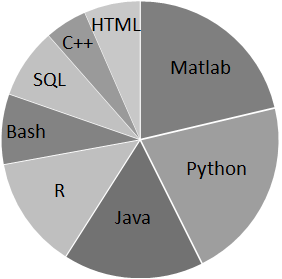
\includegraphics[scale=0.42]{img/piechart.png}
    ~
\end{aside}
\vspace{0.5cm}
\section{About}

At present, I am an early career researcher at the Big Data Institute, University of Oxford. My research interests include distributed machine learning, spatial statistics, linear mixed models, and random field theory. Most recently, I have worked on establishing probabilistic bounds for random excursion sets and introducing novel derivations for mixed model parameter estimation. 

For detailed information, publication lists, and regular updates, please visit my academic website at
\underline{\href{https://TomMaullin.com}{TomMaullin.com}}. 
\vspace{0.3cm}

\section{Academic Work}
\footnotesize{
\begin{itemize}
    \item Maullin-Sapey, T., Schwartzman, A., \& Nichols, T.E. (2023). Spatial Confidence Regions for Combinations of Excursion Sets in Image Analysis. Journal of the Royal Statistical Society Series B: Statistical Methodology 86(1). \url{https://doi.org/10.1093/jrsssb/qkad104}
    \item Maullin-Sapey, T. (2022). Multi-level Modelling and Spatial Inference for Large-Scale Neuroimaging Data. Postgraduate Thesis. \url{https://ora.ox.ac.uk/objects/uuid:425fac44-6413-47cc-b173-0a78c26aaf1c}
    \item Topiwala, A., Ebmeier, K.P., Maullin-Sapey, T., \& Nichols, T.E. (2022). Alcohol consumption and MRI markers of brain structure and function: Cohort study of 25,378 UK Biobank participants. NeuroImage: Clinical, 35, 103066. \url{https://doi.org/10.1016/j.nicl.2022.103066}
    \item Maullin-Sapey, T., \& Nichols, T.E. (2022). BLMM: Parallelised computing for big linear mixed models. NeuroImage, 264, 119729. \url{https://doi.org/10.1016/j.neuroimage.2022.119729}
    \item Maullin-Sapey, T., Schwartzman, A., \& Nichols, T. E. (2022). Spatial Confidence Regions for Conjunctions of fMRI Effects. OHBM \& RSS Conference Poster. \url{https://doi.org/10.6084/m9.figshare.21836901.v1}
    \item Maullin-Sapey, T, \& Nichols, T.E. (2021). Fisher Scoring for Crossed Factor Linear Mixed Models. Statistics and Computing, 31, 53. \url{https://doi.org/10.1007/s11222-021-10026-6}
    \item Maullin-Sapey, T., \& Nichols, T.E. (2021). BLMM: Parallelised Computing for Big Linear Mixed Models. SMI Conference Poster.\url{https://doi.org/10.6084/m9.figshare.21842097.v1}
    \item Maullin-Sapey, T., \& Nichols, T. E. (2020). BLMM: Parallelised Computing for Big Linear Mixed Models. OHBM Conference Poster. \url{https://doi.org/10.6084/m9.figshare.21842172.v1}
    \item Maullin-Sapey, T., \& Nichols, T. E. (2019). BLM: Parallelized Computing for Big Linear Models. OHBM Conference Poster. \url{https://doi.org/10.6084/m9.figshare.21842208.v1}
    \item Maullin-Sapey, T., Maumet, C., \& Nichols, T.E. (2018). Detecting and Interpreting Heterogeneity and Publication Bias in Image-Based MetaAnalyses. OHBM Conference Poster. \url{https://doi.org/10.6084/m9.figshare.21842349.v1}
    \item Maullin-Sapey, T. (2017). Visualisation and Integration of Multiple Brain Imaging Studies. Undergraduate Dissertation. \url{https://doi.org/10.6084/m9.figshare.21893061.v1}
    \item Maullin-Sapey, T. et al. (2017). Viewing FSL results with SPM and vice versa. OHBM Conference Poster. \url{https://doi.org/10.6084/m9.figshare.21861906.v1}
\end{itemize}
}
\normalsize




%  Commented out list is presentations
% \begin{itemize}
% \item Maullin-Sapey, T. (2022, November 10). \textit{BLMM: A toolbox for parameter estimation and inference on big linear mixed models on NeuroImaging data}. \textit{University of California Spatial Statistics Reading Group}. \url{https://doi.org/10.6084/m9.figshare.21892947.v1}
% \item Maullin-Sapey, T. (2022, September 13). \textit{Rapid Fire Introduction to Spatial Confidence Regions}. \textit{Royal Statistical Society Rapid Fire Sessions}. \url{https://doi.org/10.6084/m9.figshare.21892980.v1}
% \item Maullin-Sapey, T. (2022, June 6). \textit{Spatial Confidence Regions for Combinations of Excursion Sets in Image Analysis}. \textit{FMRIb Reading Group}. \url{https://doi.org/10.6084/m9.figshare.21892995.v1}
% \item Maullin-Sapey, T. (2022, June 2). \textit{Spatial Confidence Regions Methods and Proof}. \textit{University of California Spatial Statistics Reading Group}. \url{https://doi.org/10.6084/m9.figshare.21892998.v1}
% \item Maullin-Sapey, T. (2022, May 11). \textit{Tensors: What is a Tensor? (And why learn about them?)}. \textit{NISOx Reading Group}. \url{https://doi.org/10.6084/m9.figshare.21893007.v1}
% \item Maullin-Sapey, T. (2020, February 25). \textit{BLMM: A framework for distributed computation of big linear mixed models on NeuroImaging data}. \textit{FMRIb Reading Group}. \url{https://doi.org/10.6084/m9.figshare.21893010.v1}
% \item Maullin-Sapey, T. (2019, March 19). \textit{Persistent Homology: Introduction and examples}. \textit{NISOx Reading Group}. \url{https://doi.org/10.6084/m9.figshare.21893019.v1}
% \item Nichols, T., Guillaume, B. \& Maullin-Sapey, T. (2018, June 29). \textit{SwE-Toolbox: Fast and accurate modelling of longitudinal neuroimaging data}. \textit{University of Oxford}. \url{https://doi.org/10.6084/m9.figshare.21893052.v1}
% \item Maullin-Sapey, T. (2017, February 23). \textit{Visualisation and Integration of Multiple Brain Imaging Studies}. \textit{Warwick Neuroimaging Statistics Research Reading Group}. \url{https://doi.org/10.6084/m9.figshare.21893034.v1}
% \item Maullin-Sapey, T., Flandin, G., Maumet, C. \& Nichols, T. E. (2017, January 24). \textit{Reading and displaying standardised neuroimaging results in a user-friendly environment}. \textit{WIN Conference}. \url{https://doi.org/10.6084/m9.figshare.21893052.v1}
% \end{itemize}
\vspace{0.5cm}
\newpage
\newgeometry{left=2cm, right=2cm}
\section{Qualifications}

\begin{tabular}{p{0.15\linewidth} p{0.85\linewidth}}
     2018 - 2022: & \textbf{Doctoral Degree, University of Oxford:} \\
     & \\
     & My doctoral research pursued two distinct avenues of neuroimaging methods development. The first avenue focused on the derivation of novel expressions for estimation and inference of the Linear Mixed Model (LMM). These expressions were employed to perform computationally efficient large-scale fMRI LMM analyses. The second research direction centred on extending an existing theory of confidence regions to provide bounds for the intersection, or ‘conjunction’, of excursion sets that have been acquired across the same spatial region but under different study conditions. Such `conjunctions' are of natural interest in image analysis as they correspond to the question ``Where was brain activation observed in the same place across multiple study conditions?''.\\
     & \\
     2014 - 2017: & \textbf{Undergraduate Degree, University of Warwick:}\\
     & \\
     & I hold a 2:1 in BSc Data Science (Hons) from the University of Warwick. This course was comprised of modules from the Computer Science, Mathematics and Statistics programs, respectively. Through my courses, I developed a broad range of skills relevant to statistics and computing, including the ability to efficiently program in Java, R and SQL, as well as logical deduction, proof methods and the understanding and application of several widely-used statistical models.\\
    % \\
    % \underline{References:} \\ Professor Thomas Nichols (MARKER) \\Professor Armin Schwartzman (MARKER)}}
    % \\
\end{tabular}

    % \\
    % \underline{References:} \\ Professor Thomas Nichols (MARKER) \\Professor Armin Schwartzman (MARKER)}}
    % \\
 
\section{Selected Work Experience}



\begin{longtable}{p{0.15\linewidth} p{0.1\linewidth} p{0.75\linewidth}}
     2022-Present: & \multicolumn{2}{p{0.85\linewidth}}{\textbf{Post-doctorate Researcher in Neuroimaging Statistics}} \\
     & \multicolumn{2}{p{0.85\linewidth}}{\textit{Big Data Institute, University of Oxford, OX3 7LF}} \\
     & \\
     & \textbf{Roles:} & As a postdoctoral researcher, I was funded by an NIH R01 award for a project that focused on spatial confidence regions for fMRI results. During my time in this position, I have published multiple papers, attended conferences such as \textit{Organisation for Human Brain Mapping} and \textit{Royal Statistical Society}, presented posters and talks, and was actively involved in developing the grant’s renewal.  
     & \\
     & \textbf{Skills acquired:} & Experience publishing academic work, preparing grants, building research networks, strengthened knowledge of topology, probability theory and manifolds.\\
     & \\
     & \\
     2020-2022: & \multicolumn{2}{p{0.85\linewidth}}{\textbf{Graduate Teaching for Health and Data Sciences CDT programme}} \\
     & \multicolumn{2}{p{0.85\linewidth}}{\textit{Big Data Institute, University of Oxford, OX3 7LF}} \\
     & \\
     & \textbf{Roles:} & My primary role involved compiling and teaching material for the ‘Introduction to Python’ (2020, 2021 and 2022) and `Imaging with Nilearn (2021 and 2022) courses. In addition, I assisted with tutoring the ‘Modern Statistical Methods’ 2021 and ‘Data Challenge’ 2020 and 2022 courses. For the ‘Data Challenge’ held in 2020, my role additionally entailed extensive preparation and analysis of NHS Covid-19 data for the students to further investigate.\\
     & \\
     & \textbf{Skills acquired:} & Experience preparing educational content, experience teaching students across different backgrounds and with varying skill levels, effective communication skills, practical experience working with NHS Covid-19 data. \\
     & \\
     & \\
      2019-2021: & \multicolumn{2}{p{0.85\linewidth}}{\textbf{Tutoring Assistant for Interdisciplinary Bioscience CDT programme}} \\
     & \multicolumn{2}{p{0.85\linewidth}}{\textit{Doctoral Training Centre, University of Oxford,  OX1 3NP}} \\
     & \\
     & \textbf{Roles:} & In November 2019, 2020 and 2021, I helped tutor the ‘Modern Statistical Methods’ and ‘Machine Learning’ introduction courses for the Interdisciplinary Bioscience programme at Oxford. These were introductory classes for students to learn about CNN’s and regression modelling. Both classes were written in the programming language R.\\
     & \\
     & \textbf{Skills acquired:} & Teaching experience, communication skills. \\
     & \\
     & \\
      2017-2018: & \multicolumn{2}{p{0.85\linewidth}}{\textbf{Neuroimaging Research Assistant}} \\
     & \multicolumn{2}{p{0.85\linewidth}}{\textit{Big Data Institute, University of Oxford, OX3 7LF}} \\
     & \\
     & \textbf{Roles:} & Writing academic papers, creating and presenting conference posters, maintaining software.\\
     & \\
     & \textbf{Skills acquired:} & Experience with Bash, Python, CI testing and Docker containers. Understanding of random field theory, functional connectivity and time series methods used in neuroimaging. \\
     & \\
     & \\
      2016-2017: & \multicolumn{2}{p{0.85\linewidth}}{\textbf{Neuroimaging Student Intern}} \\
     & \multicolumn{2}{p{0.85\linewidth}}{\textit{International Digital Laboratory, University of Warwick, CV4 7AL}} \\
     & \\
     & \textbf{Roles:} & Developing software, providing documentation, presenting talks at conferences.\\
     & \\
     & \textbf{Skills acquired:} & Written and verbal communication skills, competency with GitHub, MatLab coding experience. \\
     & \\
     & \\
     
\end{longtable}



%%% This piece of code has been commented by Karol Kozioł due to biblatex errors. 
% 
%\printbibsection{article}{article in peer-reviewed journal}
%\begin{refsection}
%  \nocite{*}
%  \printbibliography[sorting=chronological, type=inproceedings, title={international peer-reviewed conferences/proceedings}, notkeyword={france}, heading=subbibliography]
%\end{refsection}
%\begin{refsection}
%  \nocite{*}
%  \printbibliography[sorting=chronological, type=inproceedings, title={local peer-reviewed conferences/proceedings}, keyword={france}, heading=subbibliography]
%\end{refsection}
%\printbibsection{misc}{other publications}
%\printbibsection{report}{research reports}

\end{document}
